\documentclass[11pt]{article}

\usepackage{graphicx} 
\usepackage{natbib}
\usepackage[utf8]{inputenc}

\title{Hausaufgabe 1 \\ Flussproblem}

\author{Jan Niklas Hollenbeck \\ und \\ Marco Leeske}

\date{\today}

\begin{document}

\maketitle

\newpage

\begin{abstract}

In diesem Paper wird das Flussproblem beleuchtet, welches ein mathematisches Problem zur Findung des maximalen Flusses in Netzwerken beschreibt.
 Probleme des realen Lebens werden als gerichtete Graphen modelliert und mittels gieriger Algorithmen gelöst.
 Die Anwendungsgebiete des Algorithmus sind unter anderem Kanalsysteme, Netzwerke oder Verkehrsleitsysteme.
 Zur Lösung des Flussproblems gibt es unterschiedliche Algorithmen. Diese unterscheiden sich in Laufzeit und Anwendungsfall.
 Die vorliegende Arbeit soll einen Überblick über drei verschiedene Algorithmen sowie deren  Anwendungsbereiche geben.
 Es werden die Funktionsweisen der Algorithmen von Ford und Fulkerson, Edmond und Karp wie auch des Algorithmus von Dinic erläutert, empirisch untersucht und ein Laufzeitvergleich durchgeführt.
 Dies wird mit Hilfe eines Java Programmes, welches für jeden Datensatz alle Algorithmen testet, realisiert.
 Die Daten sind nach den einzelnen Vor- und Nach-teilen der Allgorithmen ausgewählt, um auch besondere  Fälle zu testen.
 Anschließend werden die gesammelten Resultate verglichen, um sowohl eine Übersicht als auch eine Entscheidungshilfe geben zu können.
 Die Frage, welcher Algorithmus bei unterschiedlichen Ausgangssituationen und Erwartungen den Vorzug erhält, soll sich nach der Lektüre dieses Papers, so die Intention der Autoren, beantworten lassen. 

\end{abstract}


\section{Einleitung}
\label{Einleitung}

Das wird die Einleitung. Das wird die Einleitung. Das wird die Einleitung. Das wird die Einleitung. Das wird die Einleitung. Das wird die Einleitung. Das wird die Einleitung. Das wird die Einleitung. Das wird die Einleitung. Das wird die Einleitung. Das wird die Einleitung. Das wird die Einleitung. Das wird die Einleitung. Das wird die Einleitung. Das wird die Einleitung. Das wird die Einleitung. Das wird die Einleitung. Das wird die Einleitung. Das wird die Einleitung. Das wird die Einleitung. Das wird die Einleitung. Das wird die Einleitung. Das wird die Einleitung. Das wird die Einleitung. Das wird die Einleitung. Das wird die Einleitung. Das wird die Einleitung. Das wird die Einleitung. Das wird die Einleitung. Das wird die Einleitung. Das wird die Einleitung. Das wird die Einleitung. Das wird die Einleitung. Das wird die Einleitung. Das wird die Einleitung. 

%\newpage
%\tableofcontents

\newpage
\section{Einführung}
\label{Einfuehrung}

Das Flussproblem beschreibt ein mathematisches Problem in Netzwerken.

\subsection{Algorithmus}
\label{Algorithmus}

Ein Algorithmus beschreibt eine Handlungsvorschrift zur Abarbeitung eines Problems in Einzelschritten. 
\subsection{Algorithmus von Ford und Fulkerson}

\subsection{Algorithmus von Edmonds und Karp}

\subsection{Algorithmus von Dinic}

\subsection{Netzwerke}
\label{Netzwerke}



\subsection{Gerichteter Graph}
\label{Graph}

\begin{figure}[htbp] 
  \centering
     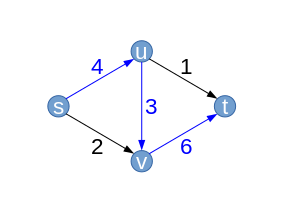
\includegraphics{graph1} 
  \caption{Bild eines Netzwerk-Graphen}
  \label{fig:Graph1}
\end{figure}

\subsection{Netzwerke}
\label{Netzwerke}

\section{Der Inhalt}
\label{Inhalt}

Flussprobleme k\"onnen in Netzwerken mithilfe von Graphen modelliert werden. Hierbei ist ein Quelle-Senke-Netzwerk(im Folgenden q-s-Netzwerk) ein kantenbewerteter, gerichteter Graph G = (V, E) mit der Eigenheit, dass eine Ecke q als Quelle sowie eine Ecke s als Senke bezeichnet wird. Die zwischen Quelle und Senke liegenden Knoten und Kanten können als Zwischenstationen aufgefasst werden. \"Uberdies wird jeder Kante, also eine Verbindung von zwei Ecken im Netzwerk, eine Kapazität c zugewiesen. Sie gibt an, wie viel maximal durch die Kante fließen kann. \citep{Testref}

In Figure \ref{fig:Graph1} unter \ref{Graph} sieht man die Senke auf der linken Seite, gekenn-zeichnet durch "S". 



\section{Experimente}
\label{Experimente}

\subsection{Wirkungsweise der Algorithmen}

\subsection{Laufzeitvergleich}

\subsection{Anwendungszenarien der jeweiligen Algorithmen}

\section{Stand der Technik (Related Work)}
\label{Related Work}
\subsection{Algorithmen und Datenstrukturen Springer Verlag}
\subsection{Graphentheoretische Konzepte und Algorithmen Vieweg und Teubner}

\section{Zusammenfassung}
\label{Zusammenfassung}
\subsection{Ausblick}



\bibliography{test}
\bibliographystyle{plainnat} 

\end{document}
